\chapter{Application sur la base d'images MNIST}
\section{Introduction}
Dans ce chapitre, nous introduisons une approche novatrice pour évaluer les performances d'un classifieur en prenant en compte la distribution de la précision. Lors de l'évaluation d'un modèle, il est essentiel de considérer la variabilité des performances d'une exécution à l'autre, notamment en fonction de l'échantillon d'apprentissage et des hyperparamètres choisis, tels que le nombre d'époques.

Pour remédier à cette problématique et obtenir une évaluation plus fiable, nous proposons d'utiliser les densités de probabilité des taux de précision comme métrique d'évaluation. Cette approche permet de prendre en compte la distribution de la précision dans l'analyse des performances du modèle.

Dans cette étude, nous appliquons cette approche à l'ensemble de données MNIST en utilisant la méthode du noyau avec l'algorithme Plug-in pour estimer les densités de probabilité des précisions de prédiction. Nous nous concentrons plus particulièrement sur l'impact du nombre d'époques sur la précision d'un classifieur CNN profond.

Pour évaluer cette influence, nous exécutons plusieurs fois le CNN en faisant varier les échantillons d'apprentissage. Cela nous permet de générer un échantillon de 100 précisions, considérées comme des réalisations indépendantes d'une variable aléatoire continue.

En utilisant la méthode du noyau avec optimisation du paramètre de lissage via l'algorithme Plug-in, nous estimons les distributions des précisions pour chaque valeur d'époque. Cette approche nous permet de comparer objectivement les performances du CNN en fonction des différentes valeurs d'époques.

En résumé, notre approche innovante consiste à évaluer les performances d'un classifieur en tenant compte de la distribution de la précision. Nous utilisons la méthode du noyau avec l'algorithme Plug-in pour estimer les densités de probabilité des précisions d'un modèle d'apprentissage automatique sur MNIST, en mettant l'accent sur l'influence du nombre d'époques sur la précision d'un CNN profond. Cette approche nous permet d'obtenir une évaluation plus objective et précise des performances du modèle.





\section{Base d'images MNIST}

Nous avons choisi la base de données MNIST pour tester notre méthode d'estimation de ddp non paramétrique. Cette base de données est bien connue dans la communauté de l'apprentissage automatique et se compose de 70 000 images de chiffres manuscrits de 0 à 9, chacune étant une image en niveaux de gris de 28 pixels sur 28 pixels.  Les images sont étiquetées avec les chiffres correspondants de 0 à 9. Cette variété d'images en fait un choix idéal pour tester la performance de notre méthode.

\begin{figure}[!h]
  \centering
  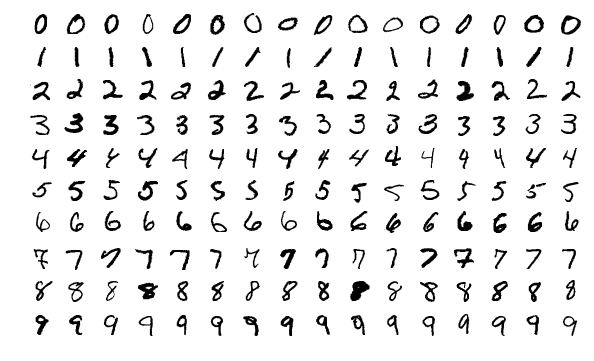
\includegraphics[width=\textwidth]{Figure 4.1.png}
  \caption{Extrait de la BD MNIST}
  \label{fig:Extrait de la BD MNIST}
\end{figure}
\clearpage 
\section{Modèle d’apprentissage}
Pour appliquer cette méthode noyau plug-in à un exemple pratique, nous avons choisi d'utiliser un modèle de réseau de neurones convolutionnel. Les CNN sont un type de modèle de ML particulièrement adapté pour les tâches de classification d'images. Les CNN ont prouvé leur efficacité dans la classification d'images en apprenant à extraire des caractéristiques pertinentes à partir des données d'entrée.

\subsection{Optimiseur: ADAM}
Dans le cas de la base de données MNIST, la nature des données est relativement simple en termes de complexité et de variabilité. Cela signifie que nous n'avons pas besoin d'un optimiseur complexe pour obtenir de bonnes performances. Cependant, ADAM (Adaptive Moment Estimation) est un choix raisonnable car il permet une convergence rapide et stable pour les modèles de réseau de neurones, ce qui est important pour obtenir une précision élevée tout en évitant le sur-apprentissage.\\ ADAM combine deux techniques d'optimisation, à savoir la méthode du gradient stochastique (SGD) et l'estimation des moments d'ordre supérieur des gradients. En utilisant ces deux techniques, ADAM peut adapter de manière adaptative le taux d'apprentissage pour chaque paramètre du modèle en fonction de son historique de gradient. En outre, ADAM maintient également une estimation des seconds moments du gradient, ce qui permet une normalisation de la mise à l'échelle des gradients et une amélioration de la convergence.

\subsection{Architecture du modèle}
Notre modèle CNN utilise 8 couches empilées les unes sur les autres :

\begin{lstlisting}
model = keras.Sequential(
        [
            keras.Input(shape=input_shape),
            layers.Conv2D(32, kernel_size=(3, 3), activation="relu"),
            layers.MaxPooling2D(pool_size=(2, 2)),
            layers.Conv2D(64, kernel_size=(3, 3), activation="relu"),
            layers.MaxPooling2D(pool_size=(2, 2)),
            layers.Flatten(),
            layers.Dropout(0.5),
            layers.Dense(num_classes, activation="softmax"),
        ]
                            )
\end{lstlisting}
\begin{figure}[!h]
  \centering
  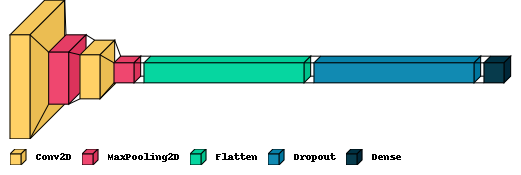
\includegraphics[width=\textwidth]{ModelView.png}
  \caption{ Model View à l'aide de Visualkeras}
  \label{fig:Model View à l'aide de Visualkeras}
\end{figure}

\begin{itemize}
    \item \textbf{La première couche}, $keras.Input(shape=inputshape)$, est une couche d'entrée qui spécifie la forme des données d'entrée. Ici, $input_shape$ correspond à la forme de chaque image d'entrée. Dans le cas de MNIST, chaque image est une matrice de 28x28 pixels en niveaux de gris, donc $inputshape=(28, 28, 1)$.
    \vspace{0.5cm}
    \item \textbf{La deuxième couche}, $layers.Conv2D(32, kernel_size=(3, 3), activation="relu")$, est une couche de convolution qui applique 32 filtres de convolution de taille 3x3 à l'image d'entrée. La fonction d'activation "relu" est utilisée pour introduire une non-linéarité dans les sorties de la couche de convolution.
        \vspace{0.5cm}
    \item \textbf{La troisième couche}, $layers.MaxPooling2D(poolsize=(2, 2))$, est une couche de pooling qui réduit la taille de la sortie de la couche de convolution en conservant uniquement la valeur maximale de chaque fenêtre de 2x2 pixels. Cette opération permet de réduire le nombre de paramètres du modèle et d'introduire une certaine invariance à la translation dans les sorties de la couche de convolution.
        \vspace{0.5cm}
    \item \textbf{La quatrième couche}, $layers.Conv2D(64, kernelsize=(3, 3), activation="relu")$, est une deuxième couche de convolution qui applique 64 filtres de convolution de taille 3x3 à la sortie de la couche de Pooling précédente.
            \vspace{0.5cm}

     \item \textbf{La cinquième  couche}, $layers.MaxPooling2D(poolsize=(2, 2))$, est une deuxième couche de Pooling qui réduit de nouveau la taille de la sortie de la deuxième couche de convolution.
         \vspace{0.5cm}
    \item \textbf{La sixième   couche}, $layers.Flatten()$, transforme la sortie de la deuxième couche de Pooling en un vecteur à une dimension, qui peut être alimenté dans des couches entièrement connectées.
        \vspace{0.5cm}
    \item \textbf{La septième couche},$layers.Dropout(0.5)$, est une couche de régularisation qui supprime aléatoirement certains neurones avec une probabilité de 0,5. Cette opération aide à prévenir le sur-apprentissage du modèle.
        \vspace{0.5cm}
     \item \textbf{La dernière   couche}, $layers.Dense(numclasses, activation="softmax")$, est une couche entièrement connectée qui calcule une probabilité pour chaque classe de sortie. Ici, $numclasses$ est le nombre de classes de sortie, qui est égal à 10 pour MNIST. La fonction d'activation "$softmax$" est utilisée pour s'assurer que la somme des probabilités pour chaque classe est égale à 1. 
\end{itemize}
\subsection{Métrique d'évaluation de la performance}
Nous avons choisi d'opter pour le taux de précision comme évaluateur de performance pour notre modèle, en raison de certaines caractéristiques importantes. Lorsque nous examinons la surface d'une densité de taux de performance, nous constatons qu'elle tend vers l'infini, ce qui indique une excellente capacité de prédiction. En revanche, la densité des taux d'erreurs tend vers zéro, ce qui suggère une faible propension à commettre des erreurs.

Cette observation nous oblige à utiliser un noyau de déformation pour garantir une bonne correspondance entre les prédictions du modèle et les valeurs réelles. Pour ce faire, nous utiliserons le taux de précision comme indicateur de performance du modèle. En utilisant un noyau conventionnel par la suite, nous pourrons mettre en œuvre les étapes nécessaires pour atteindre nos objectifs, comme nous l'expliquerons dans la section suivante.

La précision mesure le pourcentage d'images correctement classées. C’est est une métrique couramment utilisée pour évaluer les performances d'un modèle de ML. Elle mesure le nombre de prédictions correctes effectuées par le modèle sur l'ensemble des prédictions. La formule pour calculer la précision est : \\

\textbf{Précision = nombre de prédictions correctes / nombre total de prédictions}

\section{Méthodologie}
Pour évaluer la performance de notre modèle, nous avons mis en place une méthodologie rigoureuse en suivant les étapes suivantes :
\begin{enumerate}
    \item Nous avons effectué 100 itérations de l'apprentissage sur la base de données MNIST, pour chaque valeur d'époque fixe.
    \item À chaque itération, nous avons mélangé les données pour obtenir un ensemble de test différent de l'ensemble d'entraînement de la dernière itération, ce qui permet d'éviter obtention les même valeurs de précisions.
    \item À chaque itération, nous avons également stocké la valeur de la précision obtenue lors de la phase de validation dans une liste dédiée.
    \item Toutes les 100 itérations, nous avons augmenté la valeur de l'époque pour tester notre modèle avec les valeurs suivantes : [5, 10, 15, 20, 25, 30, 40].
    \item Cette procédure nous a permis d'obtenir sept listes de 100 valeurs de précision de validation pour chaque époque testée.
    \item Comme chaque liste de valeurs est considérée comme une variable aléatoire, étant donné que le mélange des données se fait de manière aléatoire et que les images dans l'ensemble d'entraînement sont également aléatoires, la précision obtenue est elle aussi aléatoire.\\ Nous avons donc appliqué la méthode de noyau Plug-in sur chacune des listes de précision (variables aléatoires) pour estimer la densité de probabilité de la précision pour les époques 5 à 40.
    \\
\end{enumerate}
\section{Résultats}
La figure ci-dessous présente les résultats de notre travail, montrant l'estimation de la densité de probabilité de la précision pour les époques 5 à 40 à l'aide de la méthode de noyau Plug-in
\clearpage
\begin{figure}[!h]
  \centering
  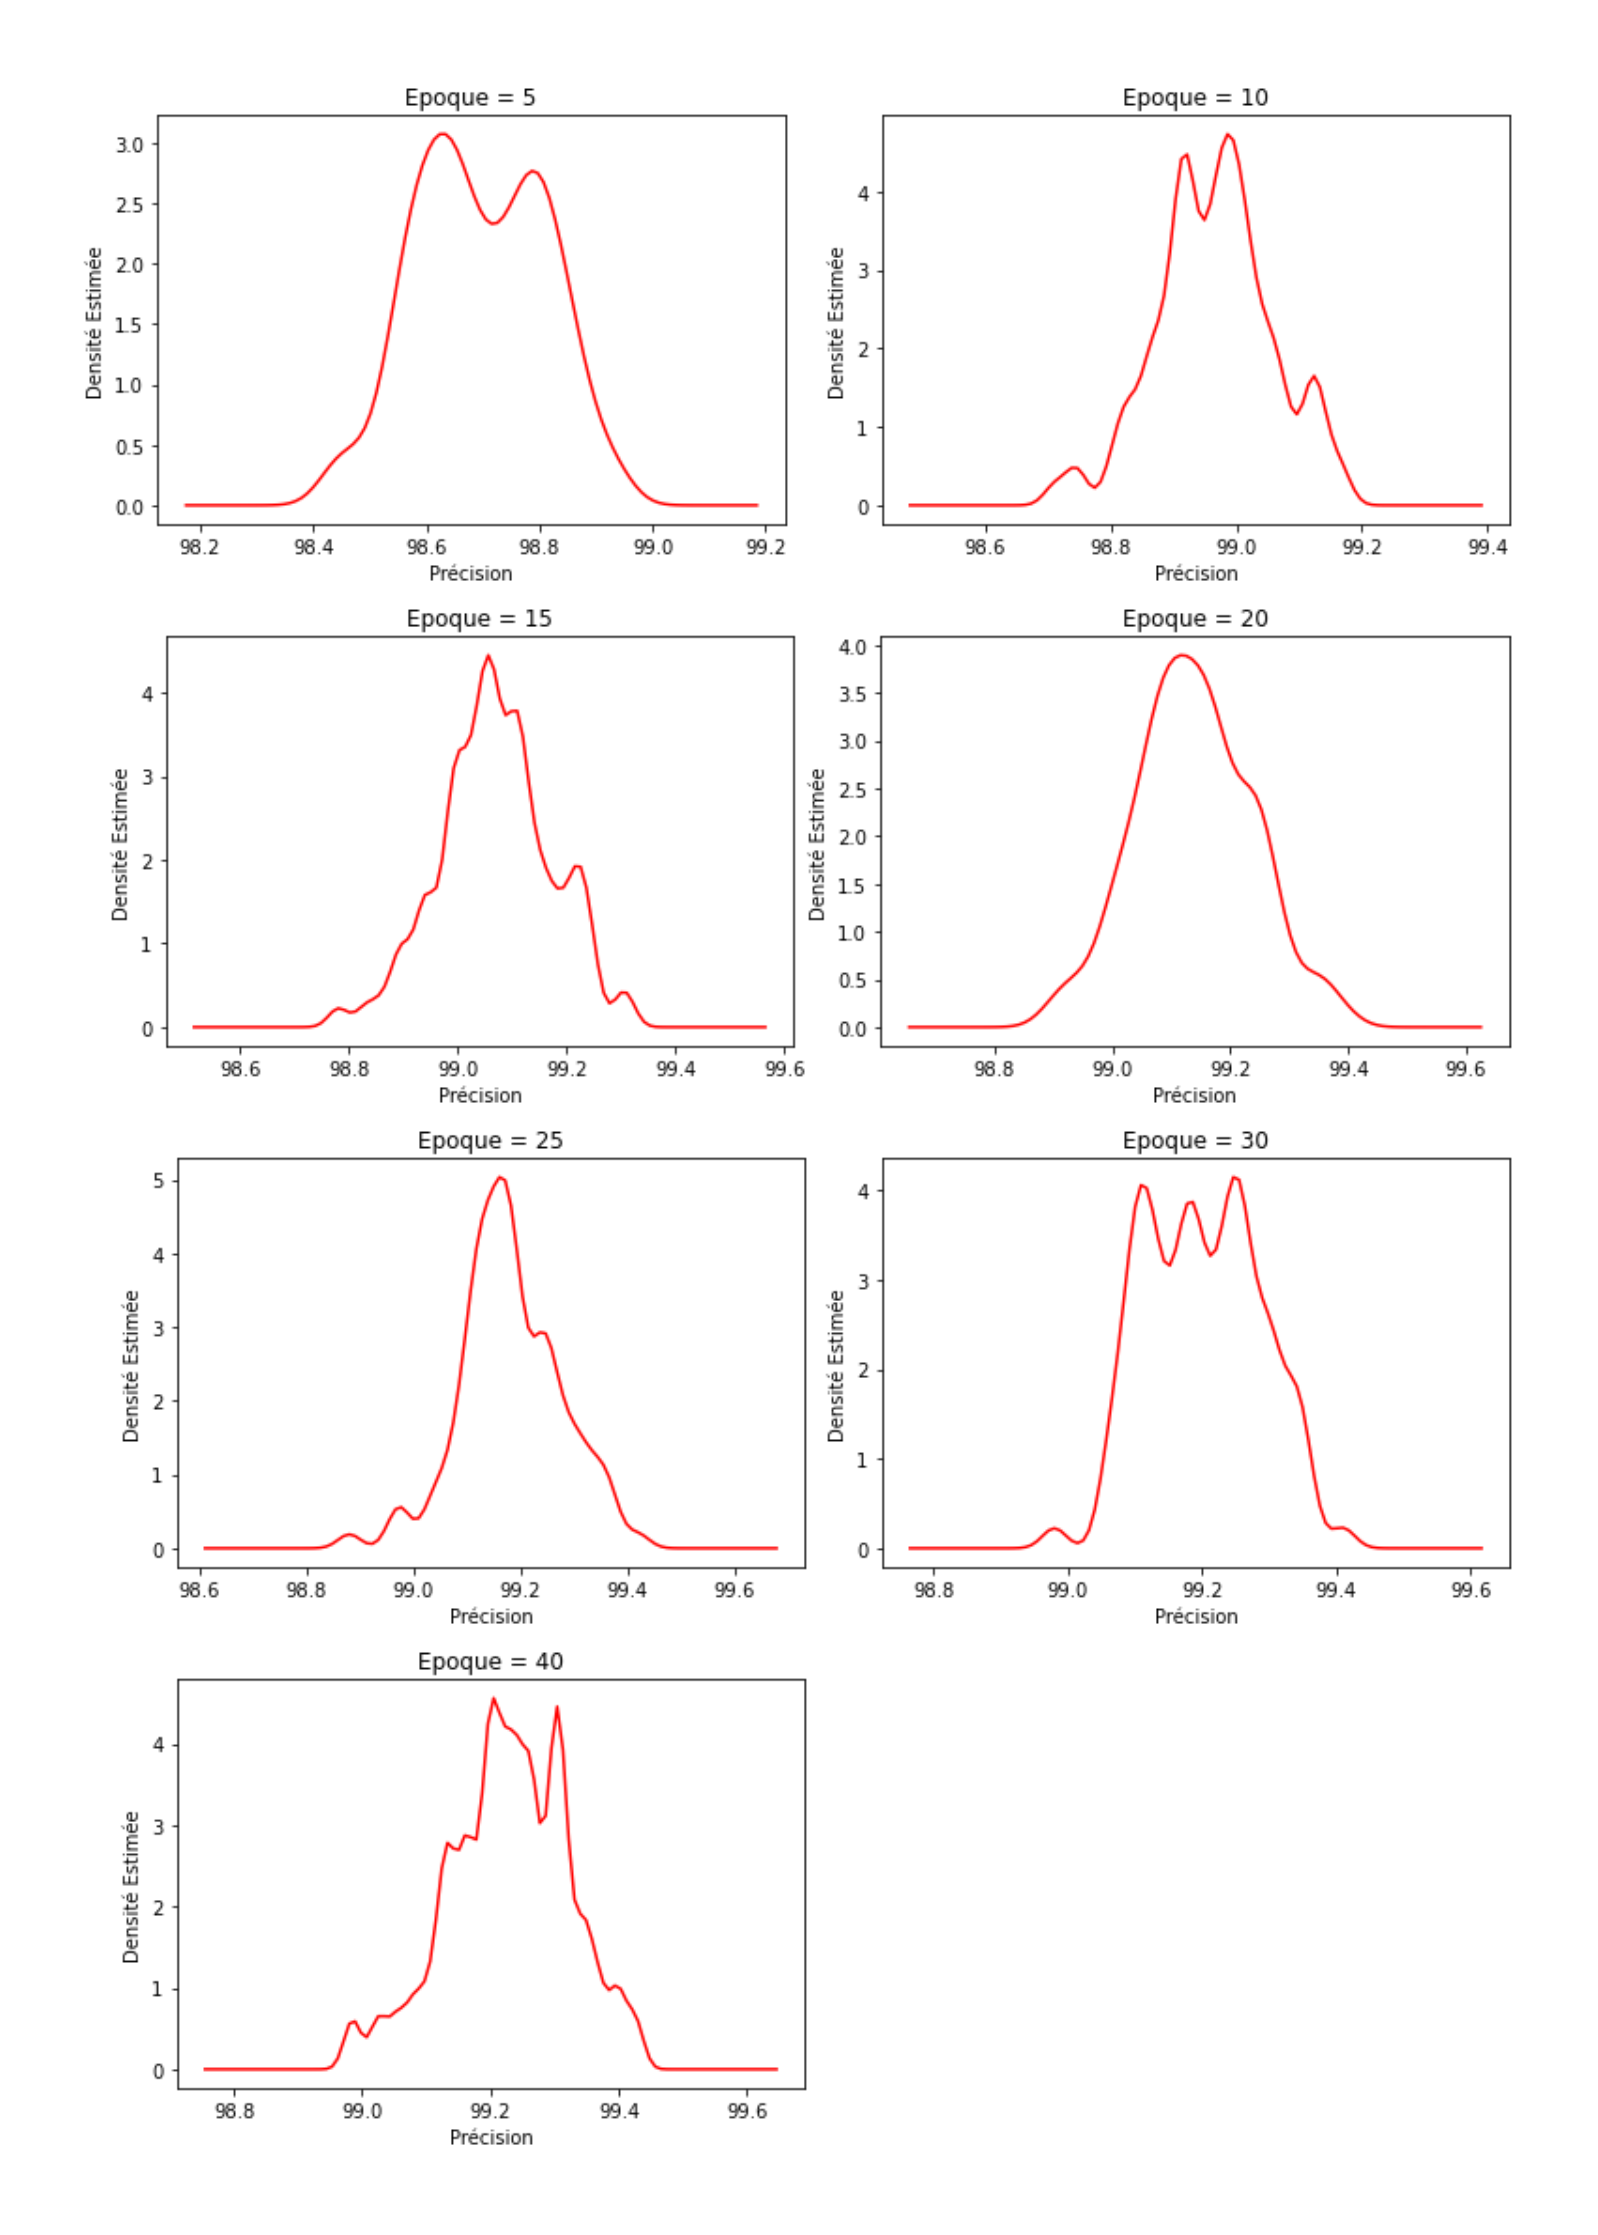
\includegraphics[width=16cm,height=21cm]{Figure 4.2.png}
  \caption{Densités estimées avec noyau Plug In}
  \label{fig:Densités estimées avec noyau Plug In}
\end{figure}
\clearpage
L'objectif de la figure suivante est de déterminer la moyenne des précisions obtenues au début et de comparer les densités par rapport à cette moyenne.

Pour ce faire, nous calculons la surface sous la courbe de densité à partir de la moyenne et en allant vers l'infini (puisque nous avons utilisé les taux de précision). Cette surface nous permet de déterminer la probabilité qu'une densité soit supérieure à la moyenne des précisions. Cette probabilité sera calculée en utilisant l'approximation des trapèzes.
\clearpage

\begin{figure}[!h]
  \centering
  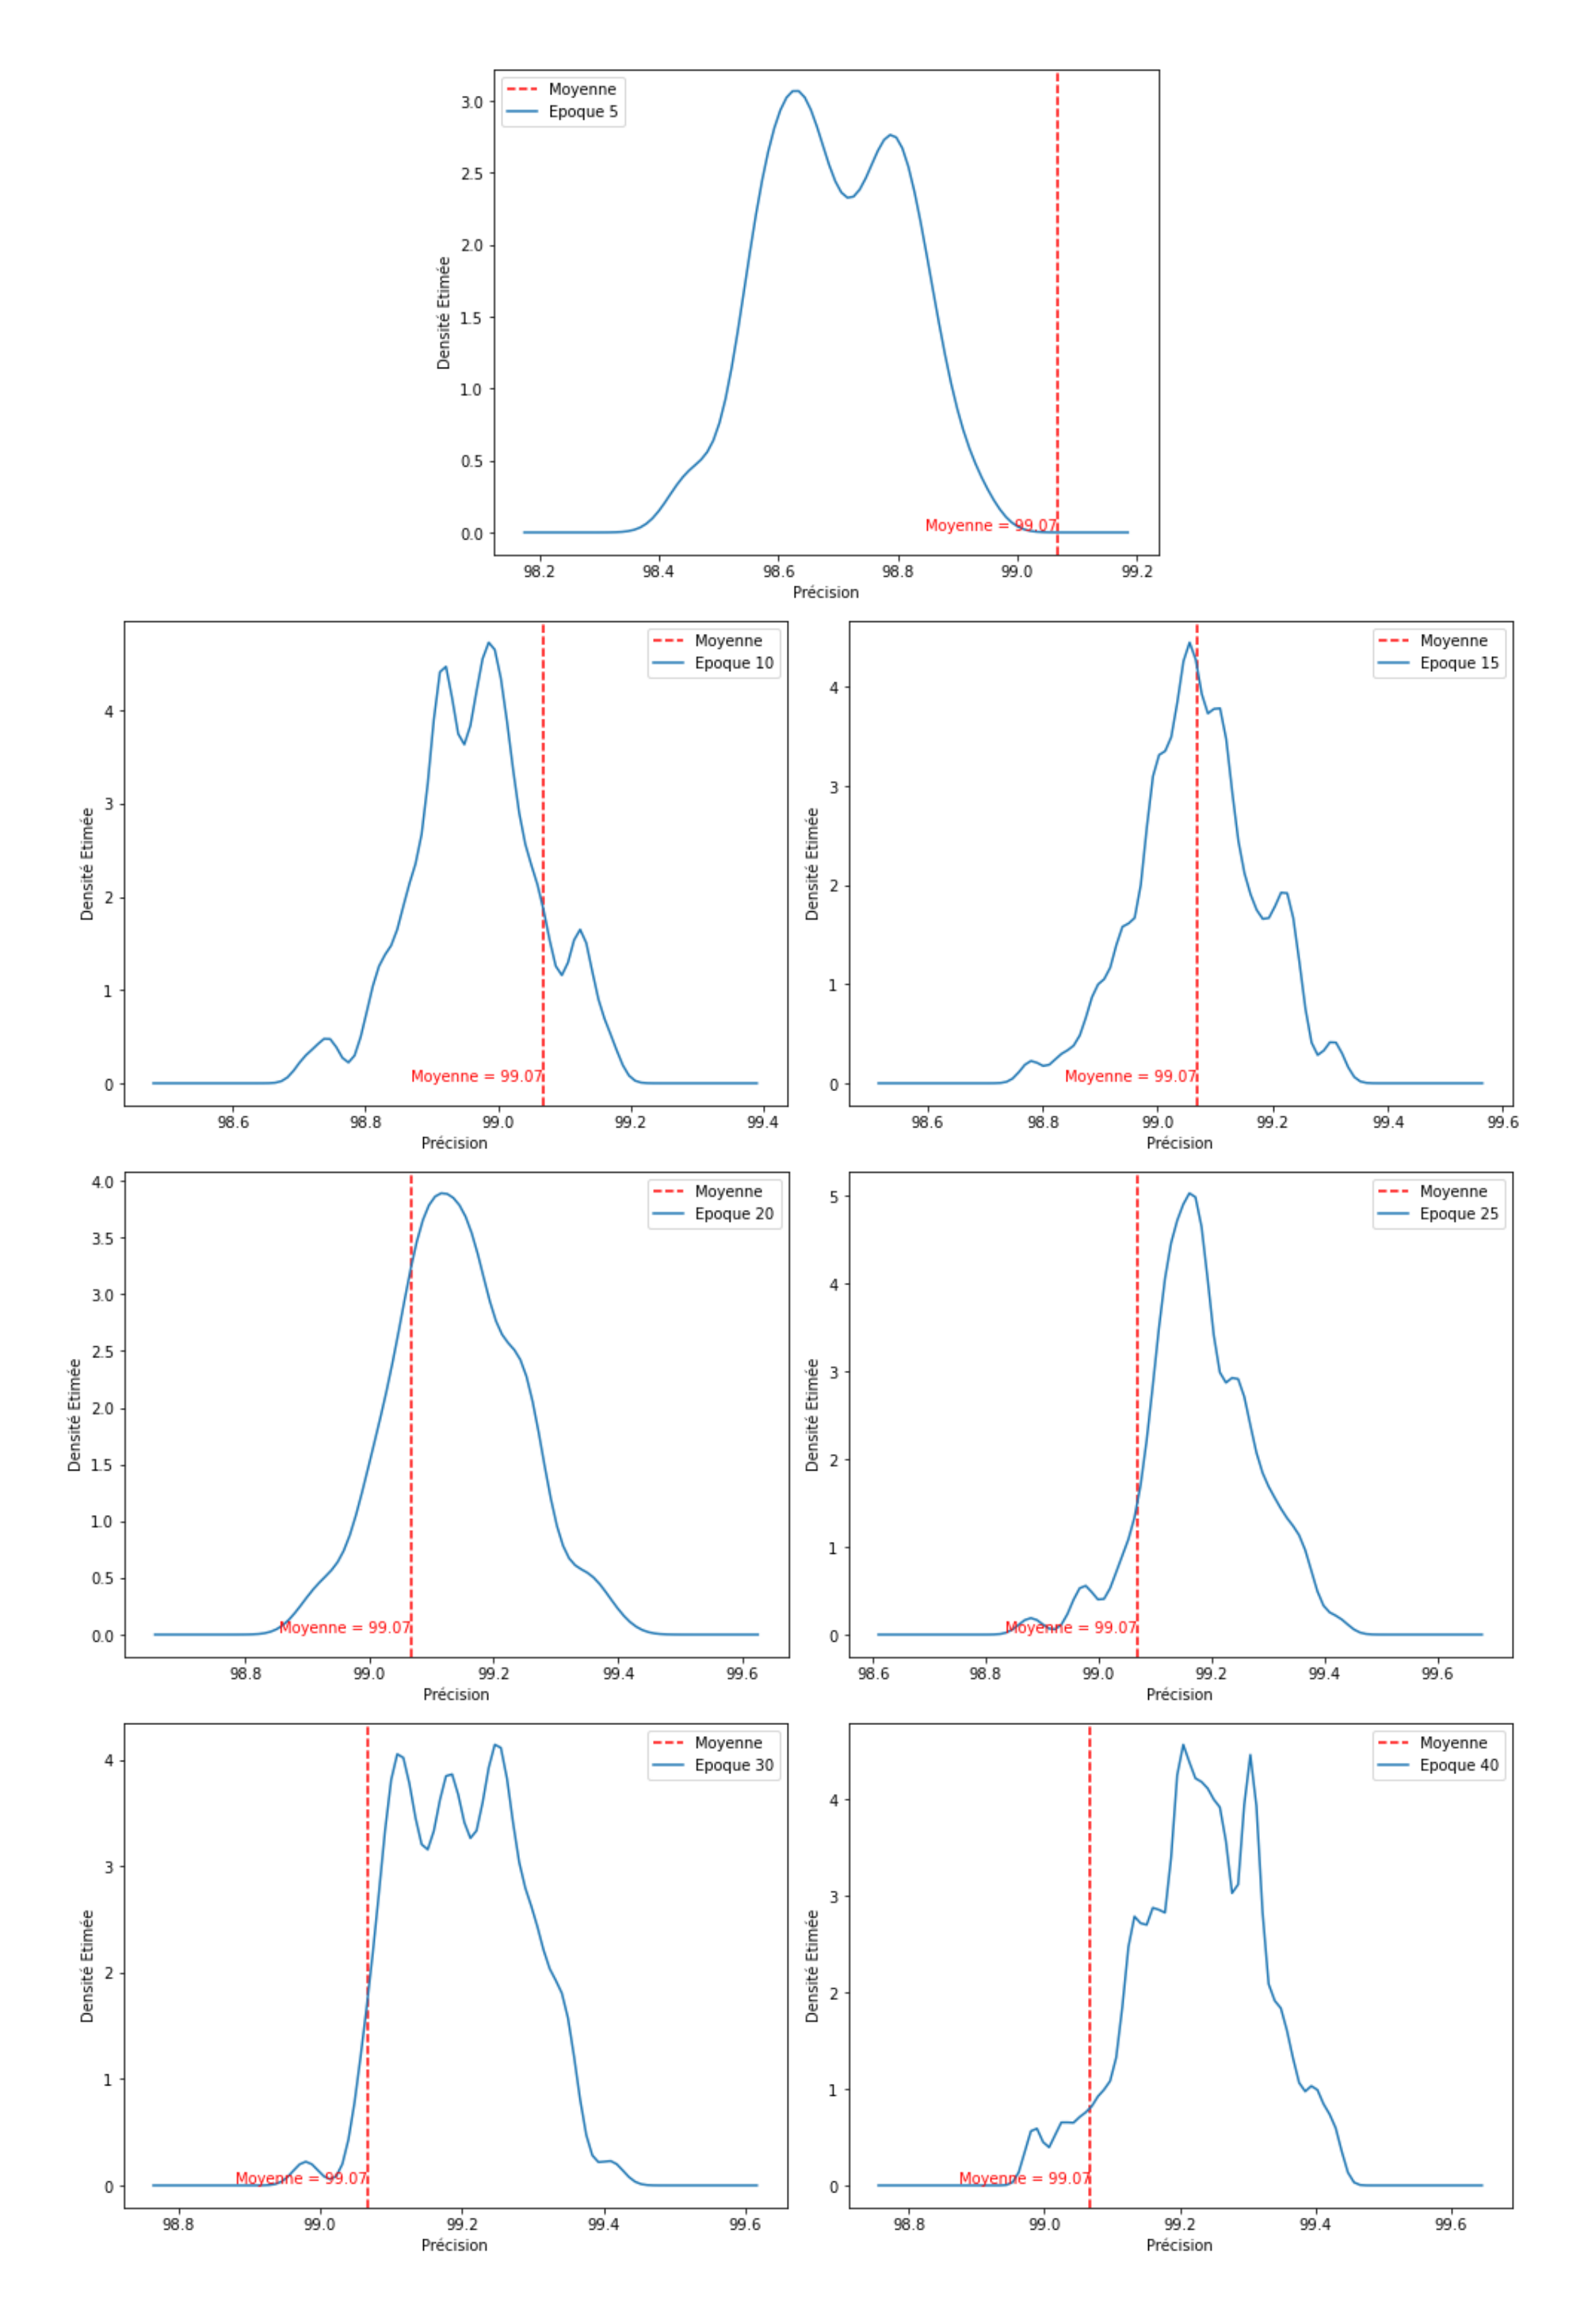
\includegraphics[width=16cm,height=21cm]{Figure 4.3.png}
  \caption{Comparaison avec la moyenne de précisions}
  \label{fig:Comparaison avec la moyenne de précisions}
\end{figure}
\clearpage
Voici une implémentation en Python 3 de la logique précédemment expliquée pour calculer la probabilité que la précision 
dépasse la moyenne des précisions : \\
$P[accuracy > m]$
\newline
Avec m : la moyenne des précisions.

\begin{lstlisting}
def calculer_surface_sous_courbe(x, y):
    # x : tableau des valeurs x de la courbe
    # y : tableau des valeurs y de la courbe

    if len(x) != len(y):
        raise ValueError("Les tableaux x et y doivent avoir la meme longueur.")

    # Calculer la surface sous la courbe par l'approximation des trapezes
    surface = np.trapz(y, x)

    return surface

num_epochs = [5, 10, 15, 20, 25, 30, 40]

for epoch in num_epochs:
    support = globals()[f"support{epoch}"] 
    epoch_sup_a_moyenne = [num for num in support if num > mean_of_means]
    deniste_sup_a_moyenne = globals()[f"Y_estimated_{epoch}"][-len(epoch_sup_a_moyenne):]

   
    print(calculer_surface_sous_courbe(epoch_sup_a_moyenne, deniste_sup_a_moyenne))
         Y[-1] = Y[-1] / (c*n*hn)
        e = -100
        d = 100
        I = 0
        Jf = 0
        z = 0
        for k in range(1, P-2):
            z = (Y[k+1]-2*Y[k]+Y[k-1])
            I += z**2
        I = I + ((Y[P-2])**2 + (Y[P-2]-2*Y[P-3])**2) / (r**4)
        #Estimation de Jf 
        Jf = I / (r**3)
        
    return Y


\end{lstlisting}
 \vspace{1cm}
 Les surfaces obtenues sont:
       \vspace{0.25cm}

 \begin{itemize}
     \item Pour le classifieur 1 ( Époque : 5 ) = $7.735e-07$ 
      \vspace{0.25cm}

    \item Pour le classifieur 2 ( Époque : 10 ) = $0.137$
      \vspace{0.25cm}

     \item Pour le classifieur 3 ( Époque : 15 ) = $0.454$ 
      \vspace{0.25cm}

     \item Pour le classifieur 4 ( Époque : 20 ) = $0.717$ 
      \vspace{0.25cm}

     \item Pour le classifieur 5 ( Époque : 25 ) = $0.887$ 
      \vspace{0.25cm}

     \item Pour le classifieur 6 ( Époque : 30 ) = $0.933$ 
      \vspace{0.25cm}

     \item Pour le classifieur 7 ( Époque : 40 ) = $0.928$ 

 \end{itemize}





\clearpage
\section{Discussion}
Dans notre expérience, nous avons étudié l'impact de différentes valeurs d'époque sur les estimations de densité des précisions pour un modèle d'apprentissage automatique entraîné sur l'ensemble de données MNIST.

En analysant les résultats, nous avons constaté que l'époque joue un rôle crucial dans la répartition de l'estimation de densité des précisions. À mesure que la valeur d'époque augmente, la densité se répartit davantage et couvre l'ensemble de l'image. Cela suggère que la précision du modèle d'apprentissage automatique s'améliore avec l'augmentation des valeurs d'époque, car le modèle est capable de capturer plus de caractéristiques dans l'ensemble de données.

Dans l'ensemble, nos estimations de densité des précisions suggèrent que l'époque=30 est la plus susceptible de produire la précision la plus élevée pour le modèle d'apprentissage automatique entraîné sur l'ensemble de données MNIST. Cette conclusion est étayée par l'utilisation de la métrique de probabilité, qui nous a permis de calculer la surface sous la courbe de densité en partant de la moyenne des précisions jusqu'à l'infini. Nous avons constaté que la densité du classifieur ayant une époque de 30 a donné la surface la plus élevée après la moyenne des précisions, ce qui suggère une précision relativement élevée et constante pour le modèle à cette époque.

En revanche, les estimations de densité pour les valeurs d'époque inférieures à 30 présentent une distribution relativement plate et diffuse, indiquant que la précision du modèle est plus variable et moins constante pour ces valeurs d'époque. De même, les estimations de densité pour les valeurs d'époque supérieures à 30 présentent des pics relativement étroits et plus bas, suggérant que la précision du modèle pourrait commencer à diminuer pour ces valeurs d'époque plus élevées.

En conclusion, nos résultats indiquent que l'époque=30 est un candidat prometteur pour atteindre une précision élevée pour le modèle CNN entraîné sur l'ensemble de données MNIST. Cependant, des analyses supplémentaires sont nécessaires pour confirmer cette conclusion et évaluer si des valeurs d'époque encore plus élevées pourraient éventuellement conduire à une diminution de la précision du modèle.
\newpage
\section{Conclusion}
En conclusion, notre étude a visé à déterminer l'époque optimale pour atteindre une précision élevée dans le modèle CNN entraîné sur l'ensemble de données MNIST. En utilisant des estimations de densité basées sur la métrique de probabilité, nous avons analysé les distributions des précisions pour différentes valeurs d'époque.

Cependant, des analyses supplémentaires sont nécessaires pour confirmer cette conclusion et évaluer si des valeurs d'époque encore plus élevées pourraient conduire à une diminution de la précision du modèle. Il est recommandé de poursuivre les recherches en examinant d'autres métriques et en effectuant des tests sur des ensembles de données supplémentaires pour une validation plus approfondie.

Dans l'ensemble, cette étude fournit des informations précieuses sur la sélection de l'époque optimale pour maximiser la précision dans le modèle d'apprentissage automatique. Ces résultats peuvent être utilisés pour améliorer les performances des modèles CNN dans diverses tâches de classification, y compris la reconnaissance de caractères et d'objets.
\newpage
\thispagestyle{empty}
\null\newpage






